\documentclass{article}
\usepackage[margin=0.5in]{geometry}
\usepackage{listings}
\usepackage{color}
\usepackage{graphicx}
\usepackage{placeins}
\usepackage{fancyhdr}
\usepackage{wrapfig}
\begin{document}
\pagestyle{fancy}
\rhead{Ryan Morehart}

\section{Task 1 - Cached Passwords}
\par Cain and Able found 6 resources on my computer. 3 of them were merely wireless keys, but 1 was actually my Lissard network password. Clearly this is sensitive information that I would not want leaked.

\section{Task 2 - Old Access Encryption}
\par Cain and Able shows the encrypted and decrypted versions of the password on the MDB almost instantly after clicking the button. I found conflicting reports on how exactly the password is stored. http://office.microsoft.com/en-us/access-help/overview-of-access-security-mdb-HP005188226.aspx states that "Microsoft Access stores the database password in an unencrypted form." However, Cain shows an encrypted version, so this can't be strictly true. Post 8 on http://www.everythingaccess.com/tutorials.asp?ID=Changing-the-encryption-type-in-Access-2007 says that Access <= 2003 used a weak implementation of the already weak RC4-32 algorithm, which seems likely to me.

\begin{figure}[h]
\centering
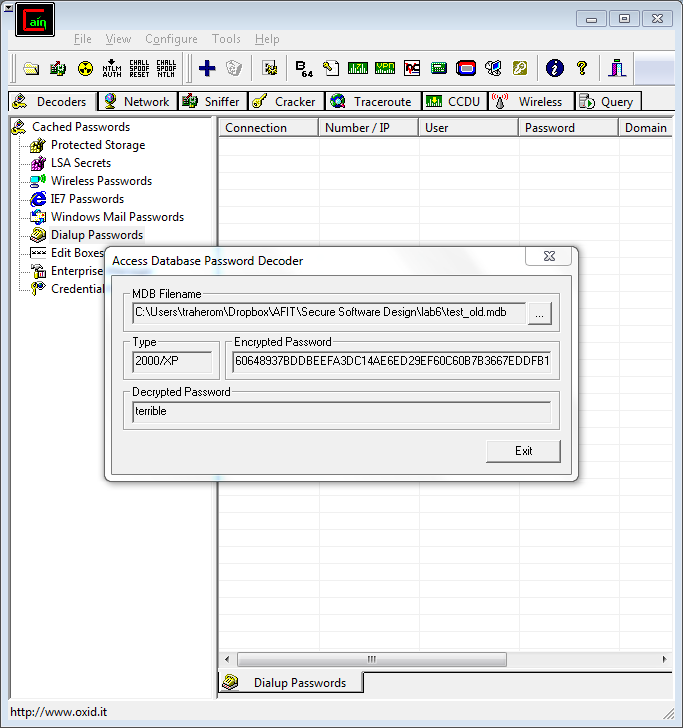
\includegraphics[width=0.78\textwidth, trim=0pt 150pt 0pt 150pt, clip]{password_broken}
\caption{Old-style MDB Password Broken}
\label{fig:mdbpwd}
\end{figure}

\section{Task 3 - New Access Encryption}
\par I used the demo version of Accdb Password Idiot Version (http://www.accdbpasswordrecovery.com/) to crack the password, after changing it to be just three numbers. As far as I can tell, this program works through mere brute force, so a stronger password provides fairly good security (esspecially when compared to MDB files).

\par According to http://www.everythingaccess.com/tutorials.asp?ID=Changing-the-encryption-type-in-Access-2007, Microsoft switched Access 2007 to use the Crypto API. Additionally, the password is not directly stored in the database and is instead just the key for the encryption. While the encryption is still not invincible, many of the weaknesses of RC4 are mitigated in various ways.

\begin{figure}[h]
\centering
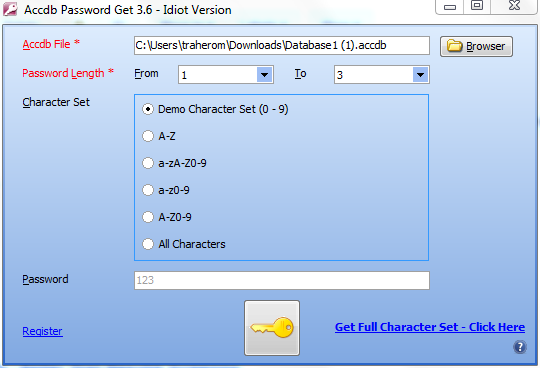
\includegraphics[width=0.78\textwidth]{2007_password_broken}
\caption{New-Style Password Broken}
\label{fig:2007_password_broken}
\end{figure}

\end{document}

